\documentclass[12pt, twoside]{article}
\input{../preamble}

\fancyhead[LO]{La Scuola d'Italia / Dr.\ Huson / IB Math: Review \\* 18 March 2026}
\fancyhead[RO]{\fbox{\begin{minipage}{6cm}\footnotesize First \& Last name:\\[0.5cm]\end{minipage}}}
\fancyfoot[C]{\thepage}

\begin{document}
\subsubsection*{11.8 Homework: Mixed Review}

\begin{center}\textbf{--- Section A: No Calculator ---}\end{center}

\begin{enumerate}[itemsep=0.15cm]

%--- Problem 1: Arithmetic sequence [5 marks] ---
\item[1.] [Maximum mark: 5]

An arithmetic sequence has $u_5 = 17$ and $u_{12} = 38$.

\begin{enumerate}[itemsep=0.1cm]
  \item Find the common difference $d$. \hfill [2]
  \item Find the first term $u_1$. \hfill [1]
  \item Find the sum of the first 20 terms, $S_{20}$. \hfill [2]
\end{enumerate}

\begin{tikzpicture}
  \draw (-0.6,0) rectangle (11,13);
  \foreach \y in {1,2,...,12} \draw[dotted] (0,\y)--(10.5,\y);
\end{tikzpicture}

\fancyhead[RO]{} % name box only on first page
\newpage

%--- Problem 2: Sector geometry [5 marks] ---
\item[2.] [Maximum mark: 5]

The following diagram shows a circle with centre O and radius 9\,cm.
Points A and B lie on the circumference. The angle
$\mathrm{A\hat{O}B} = \dfrac{2\pi}{3}$ radians.

\begin{center}
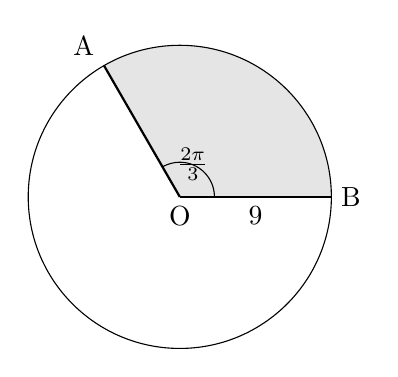
\begin{tikzpicture}[scale=0.55]
  \coordinate (O) at (0,0);
  \coordinate (B) at (3.5,0);
  \coordinate (A) at ({3.5*cos(120)},{3.5*sin(120)});
  % Shaded sector
  \fill[gray!20] (O) -- (B) arc (0:120:3.5) -- cycle;
  % Circle
  \draw (O) circle (3.5);
  % Radii
  \draw[thick] (O) -- (B);
  \draw[thick] (O) -- (A);
  % Angle arc
  \draw (0.8,0) arc (0:120:0.8);
  % Labels
  \node[above left] at (A) {A};
  \node[right] at (B) {B};
  \node[below] at (O) {O};
  \node[below] at (1.75,0) {$9$};
  \node at (0.3,0.75) {$\frac{2\pi}{3}$};
\end{tikzpicture}
\end{center}
\vspace{-0.3cm}

\begin{enumerate}[itemsep=0.1cm]
  \item Find the exact length of arc AB. \hfill [2]
  \item Find the exact area of the shaded sector. \hfill [3]
\end{enumerate}

\begin{tikzpicture}
  \draw (-0.6,0) rectangle (11,10);
  \foreach \y in {1,2,...,9} \draw[dotted] (0,\y)--(10.5,\y);
\end{tikzpicture}

\newpage

%--- Problem 3: Differentiation + tangent [5 marks] ---
\item[3.] [Maximum mark: 5]

Consider the function $f(x) = 2x^3 - x^2 + 3$.

\begin{enumerate}[itemsep=0.1cm]
  \item Find $f'(x)$. \hfill [2]
  \item Find the equation of the tangent to the graph of $f$ at $x = 1$. \hfill [3]
\end{enumerate}

\begin{tikzpicture}
  \draw (-0.6,0) rectangle (11,14);
  \foreach \y in {1,2,...,13} \draw[dotted] (0,\y)--(10.5,\y);
\end{tikzpicture}

\newpage

\begin{center}\textbf{--- Section B: Calculator Allowed ---}\end{center}

%--- Problem 4: Regression [5 marks] ---
\item[4.] [Maximum mark: 5]

The following table shows the number of hours of study ($x$) and the
test score ($y$) for seven students.

\renewcommand{\arraystretch}{1.3}
\begin{center}
\begin{tabular}{|l|c|c|c|c|c|c|c|}
    \hline
    Hours ($x$) & 2 & 3 & 4 & 5 & 6 & 7 & 8 \\
    \hline
    Score ($y$) & 48 & 55 & 58 & 70 & 74 & 82 & 85 \\
    \hline
\end{tabular}
\end{center}

The regression line of $y$ on $x$ can be written as $y = ax + b$.

\begin{enumerate}[itemsep=0.1cm]
  \item Find the value of $a$ and the value of $b$. \hfill [2]
  \item Write down the value of Pearson's product-moment correlation
        coefficient, $r$. \hfill [1]
  \item Use your regression line to estimate the test score for a student
        who studied for 5.5 hours. \hfill [2]
\end{enumerate}

\begin{tikzpicture}
  \draw (-0.6,0) rectangle (11,10);
  \foreach \y in {1,2,...,9} \draw[dotted] (0,\y)--(10.5,\y);
\end{tikzpicture}

\newpage

%--- Problem 5: Law of cosines [6 marks] ---
\item[5.] [Maximum mark: 6]

Triangle ABC has $b = 7$\,cm, $c = 10$\,cm, and
$\mathrm{B\hat{A}C} = 52^\circ$.

\begin{center}
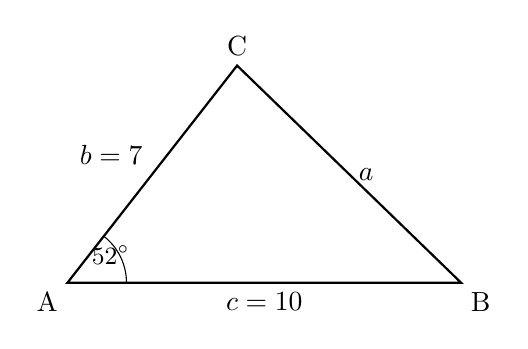
\begin{tikzpicture}[scale=0.5]
  \coordinate (A) at (0,0);
  \coordinate (B) at (10,0);
  \coordinate (C) at ({7*cos(52)},{7*sin(52)});
  \draw[thick] (A) -- (B) -- (C) -- cycle;
  % Labels
  \node[below left] at (A) {A};
  \node[below right] at (B) {B};
  \node[above] at (C) {C};
  % Side labels
  \node[below] at (5,0) {$c = 10$};
  \node[above left] at ({3.5*cos(52)},{3.5*sin(52)}) {$b = 7$};
  \node[right] at ({(10+7*cos(52))/2},{7*sin(52)/2}) {$a$};
  % Angle
  \draw (1.5,0) arc (0:52:1.5);
  \node at (1.1,0.7) {\small$52^\circ$};
\end{tikzpicture}

\textit{diagram not to scale}
\end{center}

\begin{enumerate}[itemsep=0.1cm]
  \item Find the length of side $a$. \hfill [3]
  \item Find the area of triangle ABC. \hfill [3]
\end{enumerate}

\begin{tikzpicture}
  \draw (-0.6,0) rectangle (11,10);
  \foreach \y in {1,2,...,9} \draw[dotted] (0,\y)--(10.5,\y);
\end{tikzpicture}

\newpage

%--- Problem 6: Law of sines [5 marks] ---
\item[6.] [Maximum mark: 5]

In triangle PQR, $\mathrm{Q\hat{P}R} = 40^\circ$,
$\mathrm{P\hat{R}Q} = 75^\circ$, and $p = 8$\,cm.

\begin{center}
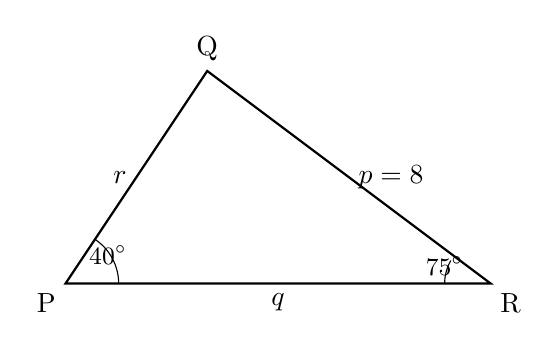
\begin{tikzpicture}[scale=0.45]
  \coordinate (P) at (0,0);
  \coordinate (R) at (12,0);
  \coordinate (Q) at ({8*cos(40)/sin(75)*sin(65)*cos(180-65-40)+ 3},{8*cos(40)/sin(75)*sin(65)*sin(180-65-40)});
  % Simpler: just place Q at a reasonable position
  \coordinate (Q) at (4, 6);
  \draw[thick] (P) -- (Q) -- (R) -- cycle;
  % Labels
  \node[below left] at (P) {P};
  \node[above] at (Q) {Q};
  \node[below right] at (R) {R};
  % Side labels
  \node[left] at (2,3) {$r$};
  \node[right] at (8,3) {$p = 8$};
  \node[below] at (6,0) {$q$};
  % Angles
  \draw (1.5,0) arc (0:56:1.5);
  \node at (1.2,0.8) {\small$40^\circ$};
  \draw ({12-1.3*cos(30)},{1.3*sin(30)}) arc (150:180:1.3);
  \node at (10.7,0.5) {\small$75^\circ$};
\end{tikzpicture}

\textit{diagram not to scale}
\end{center}

\begin{enumerate}[itemsep=0.1cm]
  \item Find the measure of angle $\mathrm{P\hat{Q}R}$. \hfill [1]
  \item Find the length of side $q$. \hfill [2]
  \item Find the area of triangle PQR. \hfill [2]
\end{enumerate}

\begin{tikzpicture}
  \draw (-0.6,0) rectangle (11,9);
  \foreach \y in {1,2,...,8} \draw[dotted] (0,\y)--(10.5,\y);
\end{tikzpicture}

\newpage

%--- Problem 7: Normal distribution [6 marks] ---
\item[7.] [Maximum mark: 6]

The weights of apples from an orchard are normally distributed with mean
150\,g and standard deviation 12\,g.

\begin{enumerate}[itemsep=0.1cm]
  \item Find the probability that a randomly chosen apple weighs less than
        165\,g. \hfill [2]
  \item Find the probability that a randomly chosen apple weighs between
        140\,g and 170\,g. \hfill [2]
  \item The heaviest 5\% of apples are classified as ``jumbo''. Find the
        minimum weight for a jumbo apple. \hfill [2]
\end{enumerate}

\begin{tikzpicture}
  \draw (-0.6,0) rectangle (11,13);
  \foreach \y in {1,2,...,12} \draw[dotted] (0,\y)--(10.5,\y);
\end{tikzpicture}

\newpage

%--- Problem 8: Compound interest [5 marks] ---
\item[8.] [Maximum mark: 5]

Olivia invests \$5000 in a savings account that pays an annual interest rate
of 3.2\%, compounded quarterly.

\begin{enumerate}[itemsep=0.1cm]
  \item Find the value of the investment after 6 years. \hfill [3]
  \item Determine how many full years it takes for the investment to
        double in value. \hfill [2]
\end{enumerate}

\begin{tikzpicture}
  \draw (-0.6,0) rectangle (11,13);
  \foreach \y in {1,2,...,12} \draw[dotted] (0,\y)--(10.5,\y);
\end{tikzpicture}

\newpage

%--- Problem 9: Probability [5 marks] ---
\item[9.] [Maximum mark: 5]

Events A and B are such that $\mathrm{P}(A) = 0.6$, $\mathrm{P}(B) = 0.5$,
and $\mathrm{P}(A \cup B) = 0.85$.

\begin{enumerate}[itemsep=0.1cm]
  \item Find $\mathrm{P}(A \cap B)$. \hfill [2]
  \item Find $\mathrm{P}(A \mid B)$. \hfill [1]
  \item Determine whether events A and B are independent.
        Justify your answer. \hfill [2]
\end{enumerate}

\begin{tikzpicture}
  \draw (-0.6,0) rectangle (11,13);
  \foreach \y in {1,2,...,12} \draw[dotted] (0,\y)--(10.5,\y);
\end{tikzpicture}

\newpage

%--- Problem 10: Binomial distribution [5 marks] ---
\item[10.] [Maximum mark: 5]

A factory produces light bulbs, and 8\% of them are defective. A quality
inspector selects 20 bulbs at random. Let $X$ be the number of defective
bulbs in the sample.

\begin{enumerate}[itemsep=0.1cm]
  \item State the distribution of $X$. \hfill [1]
  \item Find $\mathrm{P}(X = 2)$. \hfill [1]
  \item Find $\mathrm{P}(X \geq 3)$. \hfill [2]
  \item Find the expected number of defective bulbs. \hfill [1]
\end{enumerate}

\begin{tikzpicture}
  \draw (-0.6,0) rectangle (11,13);
  \foreach \y in {1,2,...,12} \draw[dotted] (0,\y)--(10.5,\y);
\end{tikzpicture}

\end{enumerate}
\end{document}

Solutions
  Problem 1 — Arithmetic sequence:
  (a) u₁₂ - u₅ = 7d = 21, d = 3
  (b) u₁ = u₅ - 4d = 17 - 12 = 5
  (c) S₂₀ = 20/2(2(5) + 19(3)) = 10(67) = 670

  Problem 2 — Sector:
  (a) Arc = rθ = 9(2π/3) = 6π cm
  (b) Area = ½r²θ = ½(81)(2π/3) = 27π cm²

  Problem 3 — Differentiation:
  (a) f'(x) = 6x² - 2x
  (b) f(1) = 2-1+3 = 4, f'(1) = 6-2 = 4
      y - 4 = 4(x - 1), y = 4x

  Problem 4 — Regression (GDC):
  (a) a ≈ 5.96, b ≈ 37.1
  (b) r ≈ 0.991
  (c) y ≈ 5.96(5.5) + 37.1 ≈ 69.9

  Problem 5 — Law of cosines:
  (a) a² = 7² + 10² - 2(7)(10)cos52° = 149 - 86.2 = 62.8, a ≈ 7.92 cm
  (b) Area = ½(7)(10)sin52° = 35(0.788) ≈ 27.6 cm²

  Problem 6 — Law of sines:
  (a) Q = 180 - 40 - 75 = 65°
  (b) q/sinQ = p/sinP → q = 8sin65°/sin40° ≈ 11.3 cm
  (c) Area = ½pq·sinR = ½(8)(11.28)sin75° ≈ 43.6 cm²

  Problem 7 — Normal distribution, X ~ N(150, 12²):
  (a) P(X < 165) = normCdf(0, 165, 150, 12) ≈ 0.894
  (b) P(140 < X < 170) = normCdf(140, 170, 150, 12) ≈ 0.749
  (c) invNorm(0.95, 150, 12) ≈ 169.7 g

  Problem 8 — Compound interest:
  (a) A = 5000(1 + 0.032/4)^24 = 5000(1.008)^24 ≈ $6053
  (b) 5000(1.008)^(4n) = 10000, (1.008)^(4n) = 2
      4n = ln2/ln1.008 ≈ 87.0, n ≈ 21.7 → 22 full years

  Problem 9 — Probability:
  (a) P(A∩B) = P(A) + P(B) - P(A∪B) = 0.6 + 0.5 - 0.85 = 0.25
  (b) P(A|B) = 0.25/0.5 = 0.5
  (c) P(A)·P(B) = 0.3 ≠ 0.25 = P(A∩B), so NOT independent

  Problem 10 — Binomial, X ~ B(20, 0.08):
  (a) X ~ B(20, 0.08)
  (b) P(X=2) = C(20,2)(0.08)²(0.92)^18 ≈ 0.271
  (c) P(X≥3) = 1 - P(X≤2) ≈ 1 - 0.790 ≈ 0.210
  (d) E(X) = 20(0.08) = 1.6
